\section{Results}
\label{sec:results}

All results are reported at the second rescripting turn (slice~2), aggregated across six vignettes. Statistics are computed over 390 experiment runs (13 models $\times$ 6 vignettes $\times$ 5 temperatures, 20 trials each). Tests are exploratory. Kruskal--Wallis $H$ is reported with $\eta^2$ effect sizes, and pairwise contrasts use Mann--Whitney $U$ with Bonferroni correction over $\binom{13}{2}=78$ comparisons.

\subsection{Plan Validity and Strategy Distribution}
\label{sec:validity}

Before analysing stability, the plan extraction step must be validated. The structured format turns out to be essentially free: overall validity is 99.8\%, with every model at or above 98.3\% (Command~A lowest; Figure~\ref{fig:validity}), and validity does not vary meaningfully with temperature. The fused prompt reliably elicits structured plan output, and the stability metrics below are computed over near-complete data. The seventeen malformed trials are treated as missing data (Section~\ref{sec:metrics}).

Across 15{,}561 declared strategy picks, all six taxonomy categories are used, though not uniformly: \texttt{sensory\_modulation} (27.1\%), \texttt{cognitive\_reframe} (24.2\%), and \texttt{self\_empowerment} (21.9\%) dominate, while \texttt{safety} (9.9\%), \texttt{social\_support} (9.6\%), and \texttt{confrontation} (7.3\%) form a long tail (Figure~\ref{fig:strategies}). No category exceeds a third of picks, in contrast to the 87.7\% single-category skew of the initial taxonomy (Appendix~\ref{app:taxonomy}).

These distributional differences are a prerequisite for interpreting the consistency results that follow. A model that always selects the same two strategies will score high on Jaccard regardless of temperature, while a model with a wider repertoire has more room to vary. Mistral Large~4 concentrates most (77\% of picks in its top two categories), followed by OLMo~3.1~32B (73\%) and Qwen~3.5~122B (71\%). Large~4 never selects confrontation (0 of 1{,}200 picks). The proprietary models follow (65--67\%), and Command~A, Mistral Large~3, and Mistral Small~4 spread widest (46--49\%).

\begin{figure}[t]
  \centering
  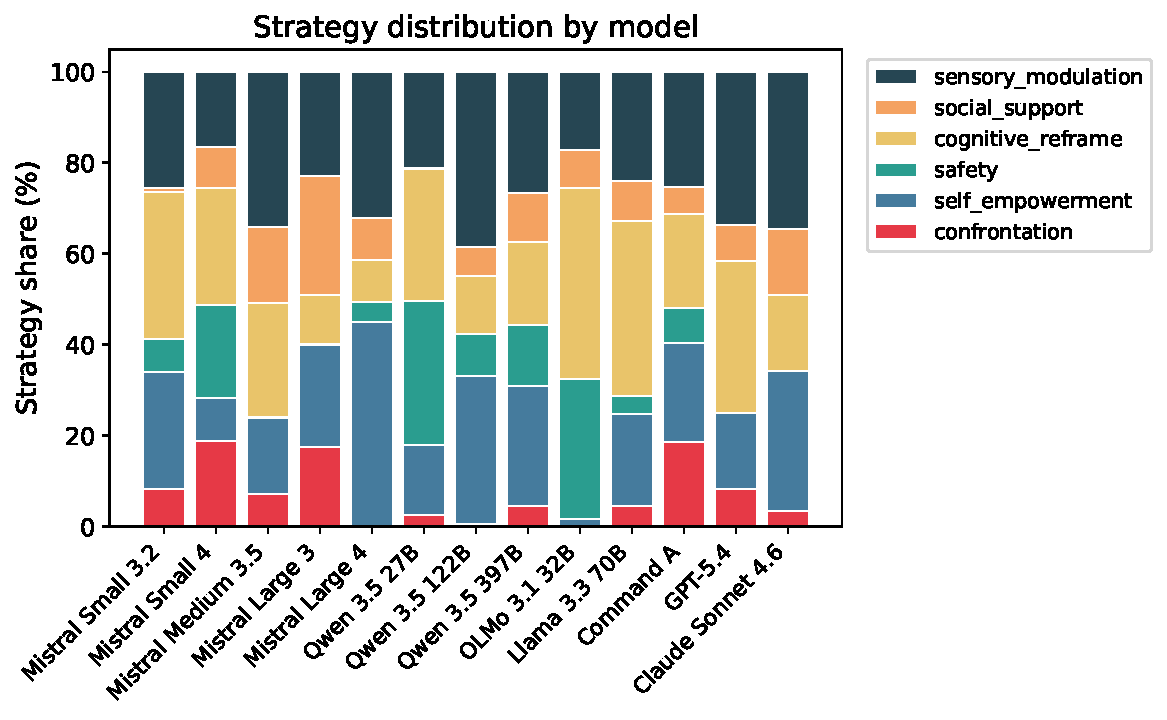
\includegraphics[width=.95\linewidth]{fig_5_1_strategy_distribution}
  \caption{Strategy distribution by model, pooled across temperatures and vignettes. Each bar shows the share of trials selecting each taxonomy category. Models with narrower distributions have less room to vary.}
  \label{fig:strategies}
\end{figure}

\subsection{Plan Consistency (Method 1)}
\label{sec:results-jaccard}

Figure~\ref{fig:jaccard} presents the headline result: decision-level stability is high but far from universal. Median pairwise Jaccard per run ranges from 1.000 (GPT-5.4, Mistral Large~4, Mistral Medium~3.5, Mistral Small~3.2, OLMo~3.1~32B, Qwen~3.5~122B) down to 0.689--0.727 (Qwen~3.5~397B, Llama~3.3~70B, Qwen~3.5~27B). Even at fixed temperature and identical context, the least stable models change their declared therapeutic strategy in roughly one of three trial pairs.

\begin{figure}[t]
  \centering
  \makebox[\textwidth]{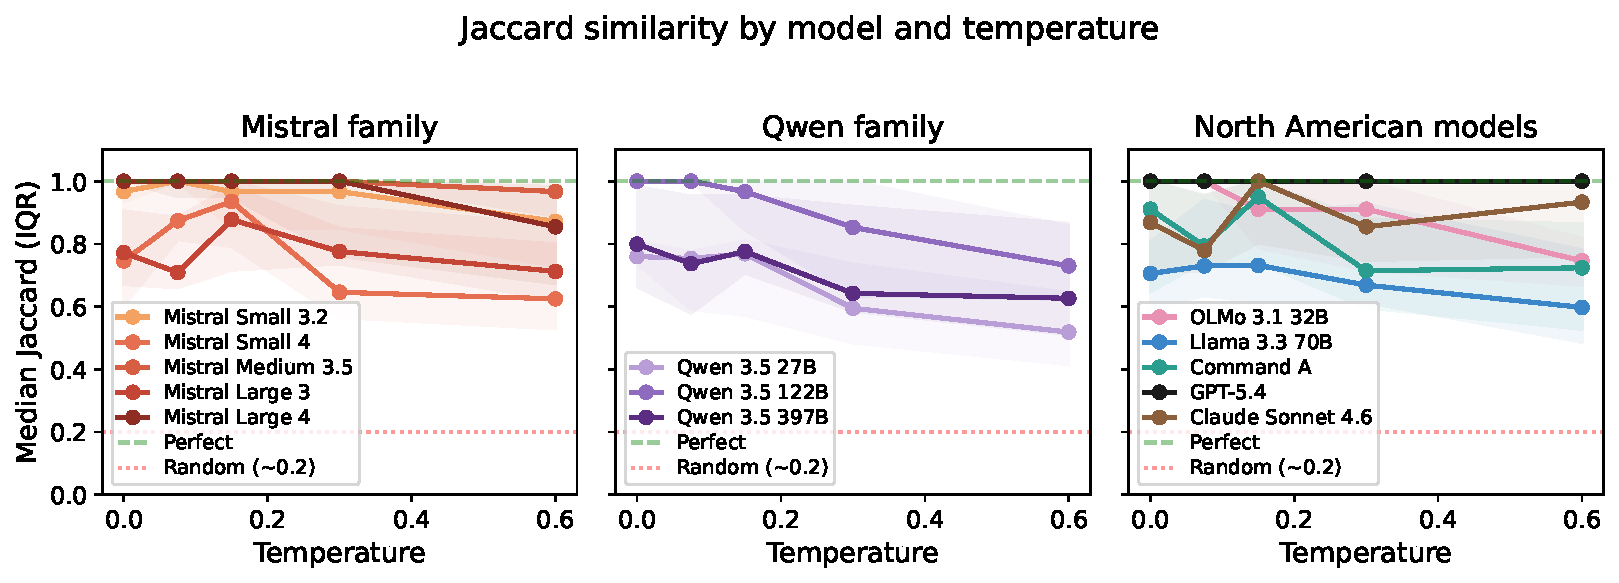
\includegraphics[width=1.12\textwidth]{fig_5_2_jaccard}}
  \caption{Median pairwise Jaccard by model and temperature, grouped by family. Shaded bands show IQR. The dashed line marks perfect consistency, the dotted line the random baseline ($J \approx 0.2$). Higher is more consistent.}
  \label{fig:jaccard}
\end{figure}

Temperature degrades decision consistency overall (pooled Spearman $\rho=-0.220$, $p<.001$; Kruskal--Wallis $H(4)=24.1$, $p<.001$, $\eta^2=0.062$): the grand median falls from 1.000 at $T{=}0.0$ to 0.767 at $T{=}0.6$. But the effect is far from uniform. Per-model correlations separate three groups: OLMo~3.1~32B ($\rho=-0.65$), Qwen~3.5~122B ($\rho=-0.56$), and Qwen~3.5~27B ($\rho=-0.49$) degrade significantly, the Mistral family and Command~A show no significant trend, and the proprietary ceilings are flat ($\rho=+0.03$ for Sonnet~4.6, $+0.09$ for GPT-5.4). The most capable models hold their therapeutic decisions stable across the whole sampled range.

Greedy decoding, however, is not always optimal. Ten of the thirteen models reach their best mean Jaccard at a non-zero temperature. The pattern is clearest in the Mistral family: Mistral Small~4 rises from 0.777 at $T{=}0.0$ to 0.881 at $T{=}0.15$, Mistral Large~3 from 0.796 to 0.848 at $T{=}0.15$, and Llama~3.3~70B from 0.719 to 0.775 at $T{=}0.075$. The first two post-hoc additions follow the same pattern: Mistral Medium~3.5 peaks at a perfect 1.000 mean at $T{=}0.075$, above its 0.979 at $T{=}0.0$, and Command~A rises from 0.832 to 0.861 at $T{=}0.15$. Mistral Large~4 does not: its mean is highest at $T{=}0.0$ (0.956) and lowest at $T{=}0.6$ (0.818). Whether these differences reflect a genuine benefit of low sampling variance or sample variation ($n=6$ vignettes per cell) cannot be determined from these results alone, but they are consistent with Mistral's vendor default of $T{=}0.15$.

Model differences are substantial (Kruskal--Wallis $H(12)=109.6$, $p<.001$, $\eta^2=0.282$; 22 of 78 Bonferroni-corrected pairs significant). Modal-set agreement, the fraction of trials whose declared set equals the run's most common set and thus a per-trial statistic free of the pairwise dependence noted in Section~\ref{sec:metrics}, tells the same story (Figure~\ref{fig:modal} in Appendix~\ref{app:modal}), from 0.993 (GPT-5.4) and 0.972 (Mistral Medium~3.5) down to 0.670 (Qwen~3.5~27B).

\subsection{Response Similarity (Method 2)}
\label{sec:results-bertscore}

BERTScore F1 measures semantic similarity between the response texts, independent of the plan block. The pooled temperature effect is roughly twice as strong as for Jaccard ($\rho=-0.499$, $p<.001$; $H(4)=104.6$, $p<.001$, $\eta^2=0.269$), with the median falling from 0.787 at $T{=}0.0$ to 0.705 at $T{=}0.6$ (Figure~\ref{fig:bertscore}). Rising temperature changes response wording before it changes strategy selection: models say the same thing differently before they decide differently.

BERTScore is, however, largely insensitive to strategy changes. A model that switches from \emph{confrontation} to \emph{cognitive reframe} produces surface text similar enough that BERTScore barely registers the difference, since different rescripting strategies share the same conversational framing, sentence length, and register. A per-pair analysis over all 68{,}400 trial pairs of the original 360 runs quantifies this. Pairs with identical strategy sets average F1 0.78 against 0.61 for pairs with fully disjoint sets, and within a single model the gap is typically near 0.1, about the size of the buckets' standard deviations. The distributions overlap too heavily for any BERTScore threshold to separate a strategy switch from a change in wording. BERTScore therefore serves as a check on response style rather than as a measure of decision stability. Between-model differences are again large ($H(12)=92.0$, $p<.001$, $\eta^2=0.237$; 20 of 78 pairs significant), with Mistral Medium~3.5 highest (mean F1 0.816) and Mistral Small~4 lowest (0.697).

\begin{figure}[t]
  \centering
  \makebox[\textwidth]{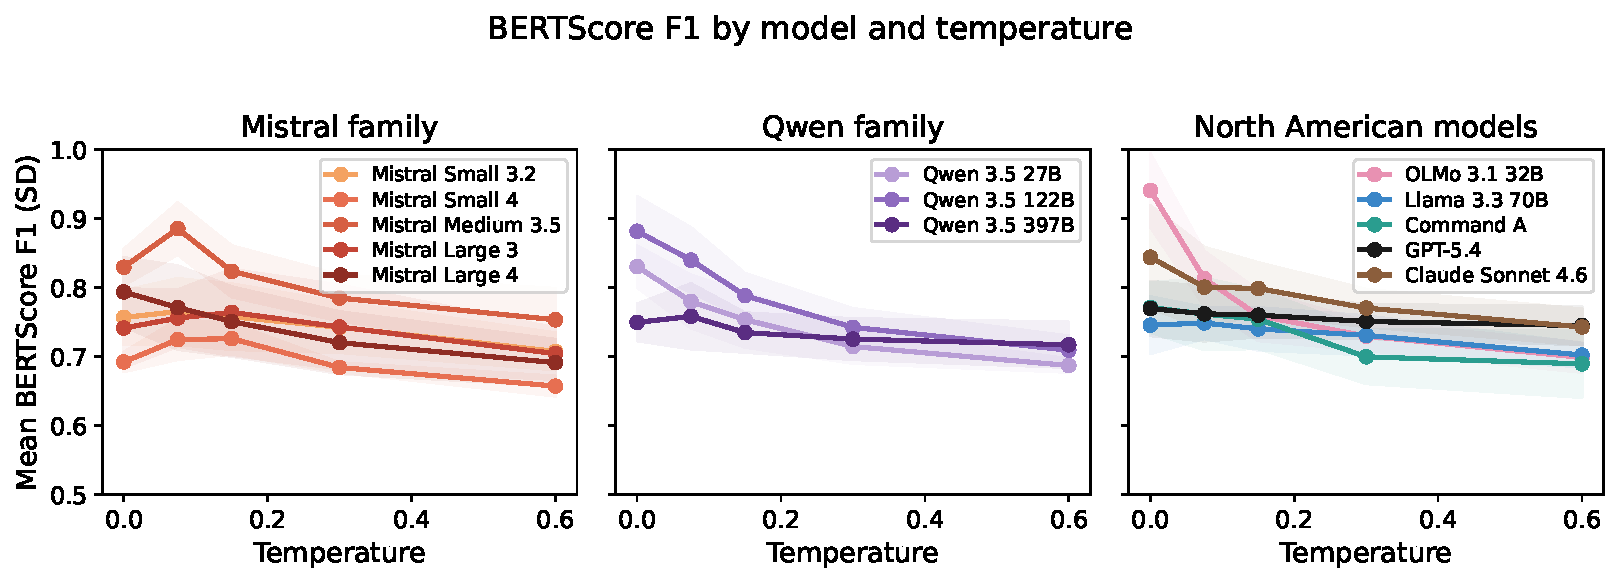
\includegraphics[width=1.12\textwidth]{fig_5_3_bertscore}}
  \caption{Pairwise BERTScore F1 by model and temperature, grouped by family.}
  \label{fig:bertscore}
\end{figure}

\subsection{Vignette Effects}
\label{sec:results-vignettes}

The data show no evidence that patient presentation drives stability. Vignette differences are significant for neither decision consistency ($H(5)=5.4$, $p=.370$, $\eta^2=0.014$) nor response similarity ($H(5)=10.1$, $p=.072$, $\eta^2=0.026$), although the latter comes closer: patient profile affects response wording more than strategy selection. Median Jaccard spans a narrow 0.821 (cooperative, resistant) to 1.000 (anxious, skeptic). With six vignettes the test is underpowered, so this is an absence of evidence for a vignette effect rather than evidence of invariance. Individual model--vignette combinations do deviate from the aggregate, which keeps per-vignette reporting useful for spotting where a specific model breaks down. The full per-vignette heatmaps appear in Appendix~\ref{app:vignettes}.

\subsection{Cross-Metric Relations}
\label{sec:results-correlations}

The three methods are related but not redundant. Decision- and response-level consistency correlate moderately (Spearman $\rho=0.543$, $p<.001$, $n=390$): models with more consistent strategy selection also tend to produce more similar text, but not strongly enough for one metric to substitute for the other. Alignment correlates only weakly with Jaccard ($\rho=0.245$) and moderately with BERTScore ($\rho=0.382$), consistent with its role as a near-ceiling validation check rather than a third stability axis.

Figure~\ref{fig:correlations} shows how the models arrange on the two stability axes. Mistral Medium~3.5 anchors the upper right, six models sit at perfect median decision consistency with clearly different response-level scores, and Qwen~3.5~27B occupies the lower left. Mistral Small~4 presents an interesting case: moderate decision consistency but the lowest response similarity in the set, so even when it selects the same strategies, its wording varies considerably.

\begin{figure}[t]
  \centering
  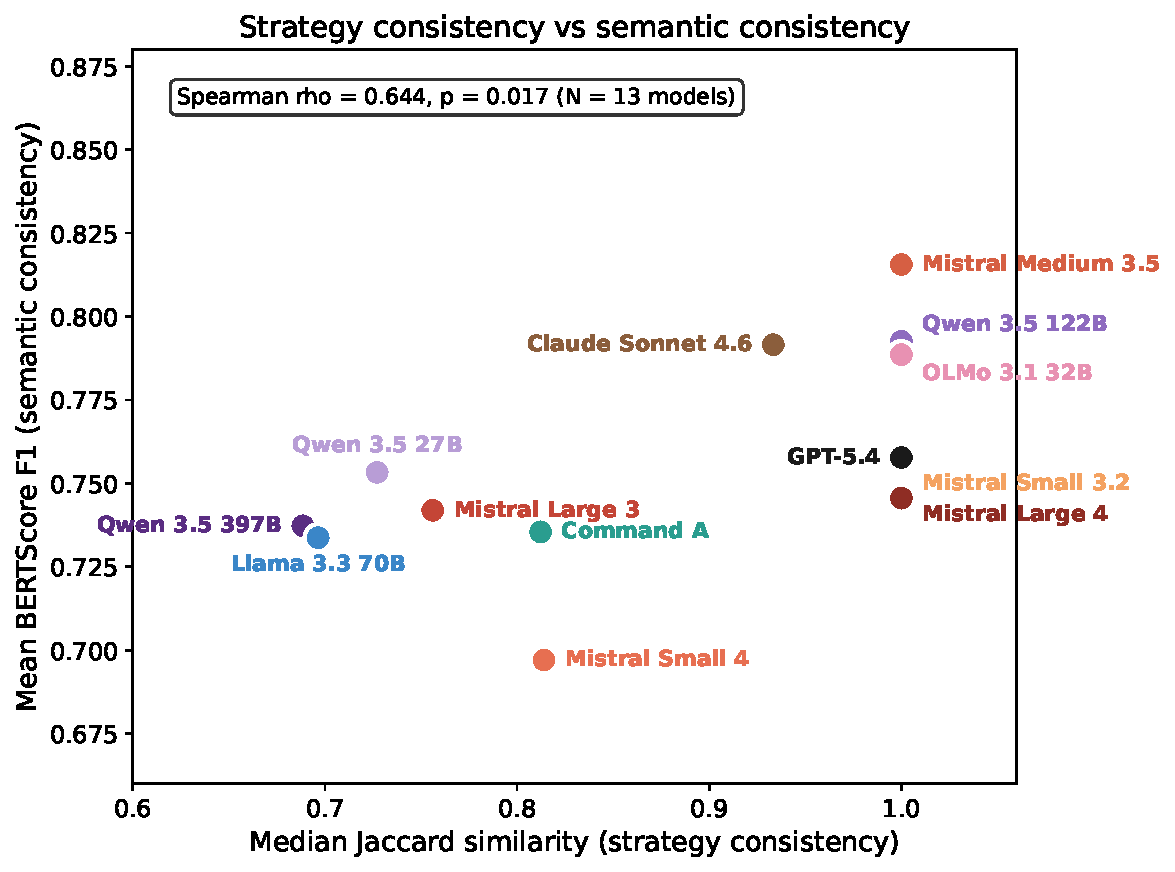
\includegraphics[width=.82\linewidth]{fig_5_5_correlations}
  \caption{Plan consistency (median Jaccard) versus response similarity (mean BERTScore F1) per model, pooled across temperatures and vignettes.}
  \label{fig:correlations}
\end{figure}

\subsection{Plan--Response Alignment (Method 3)}
\label{sec:results-alignment}

Models largely do what they declare. Mean alignment ranges from 1.000 (GPT-5.4 and Sonnet~4.6) down to 0.810 (Mistral Small~4), and it is temperature-independent ($\rho=-0.058$, $p=.25$). Models do not get worse at implementing their declared strategies as temperature rises: they select \emph{different} strategies more often (lower Jaccard) but implement whichever strategy they select equally well (Figure~\ref{fig:alignment}).

Model differences on alignment are nonetheless the largest of the three metrics ($H(12)=164.9$, $p<.001$, $\eta^2=0.424$; 38 of 78 pairs significant), driven by the gap between the proprietary ceilings (1.000) and the weaker open models. The near-ceiling scores validate Method~1: declared plans are implemented, so Jaccard measures genuine decision variability rather than label noise. Judge accounting: of 7{,}800 trials, none failed with judge errors, 17 were unjudgeable (invalid plans, 10 of them Command~A's, excluded as missing data), and 9 trials (0.12\%) were re-judged by the Gemini~3.1 Pro fallback.

\begin{figure}[t]
  \centering
  \makebox[\textwidth]{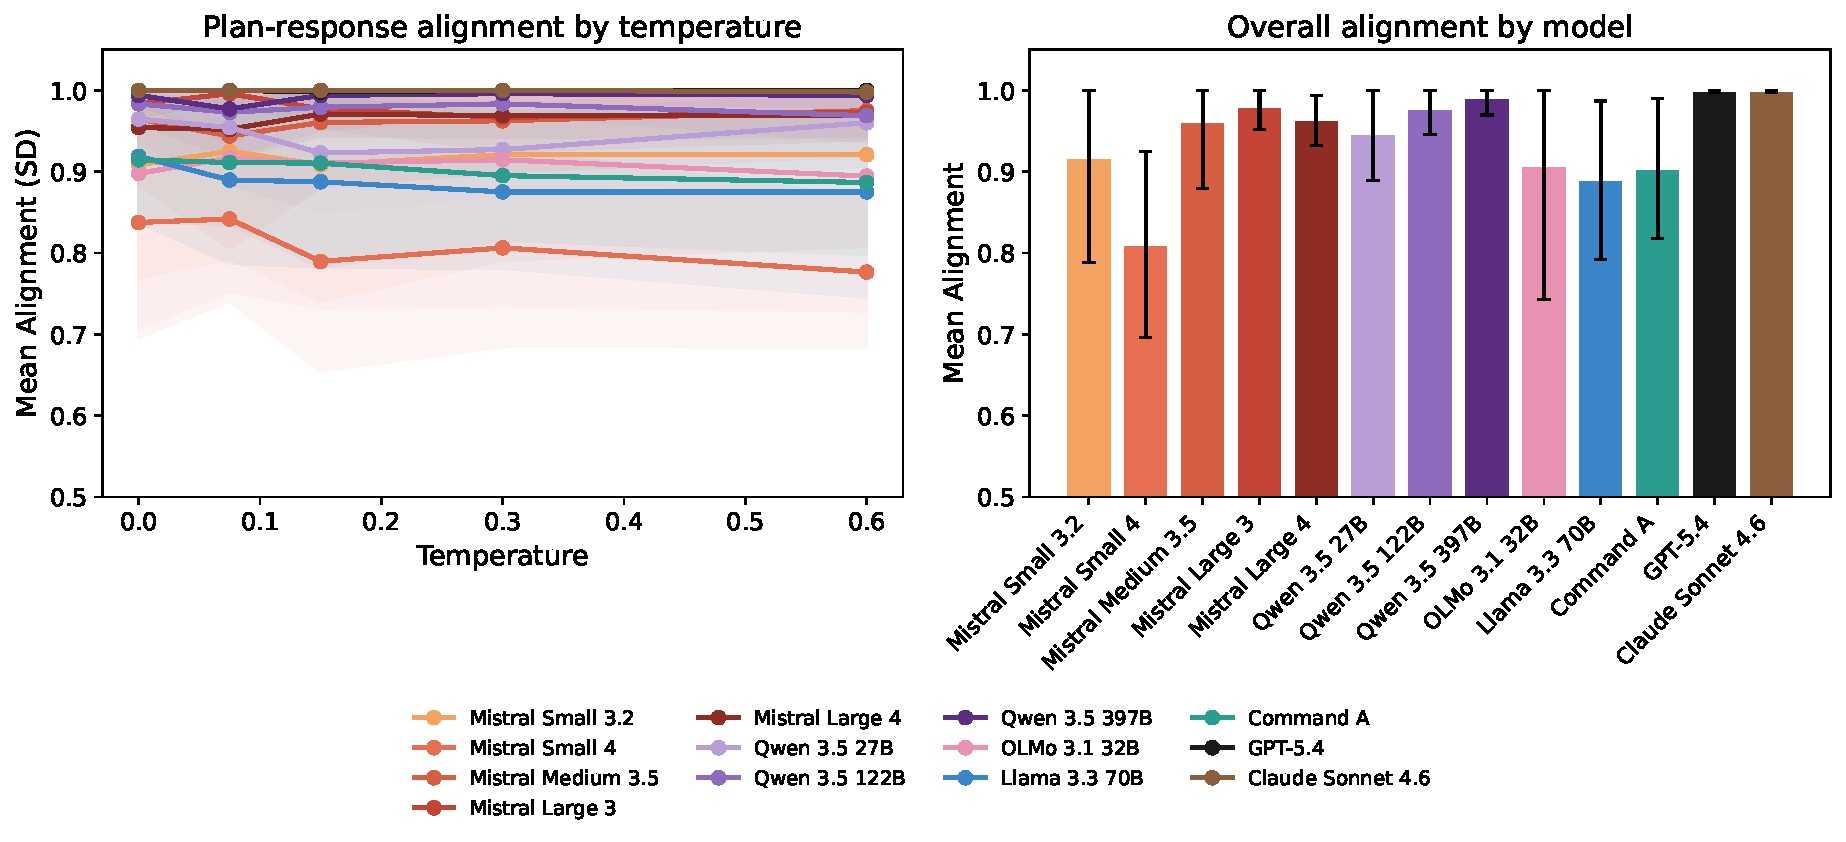
\includegraphics[width=1.05\textwidth]{fig_5_6_alignment}}
  \caption{Plan--response alignment by model.}
  \label{fig:alignment}
\end{figure}

\subsection{Robustness to Model-Set Changes}
\label{sec:robustness-results}

The first post-hoc addition lands at the top of the stability ranking. Mistral Medium~3.5 attains a perfect median Jaccard of 1.000, the highest mean BERTScore F1 in the set (0.816), the second-highest modal-set agreement (0.972), perfect plan validity, and mean alignment of 0.961 across its 30 conditions. Its Jaccard profile stays at or near ceiling across all five temperatures. This ceiling is not the sampling artefact diagnosed for GPT-5.4 below: Medium~3.5's BERTScore falls by 0.13 across the sweep ($\rho=-0.66$), the steepest response-level temperature reaction among the top-ranked models, so temperature demonstrably reaches the model and it is the decisions that hold still while the wording drifts. Its consistency does not come from a narrow repertoire either: its pooled strategy distribution is broader than that of the proprietary models (59\% top-two share), so its selections vary across patients but not across runs of the same patient.

The second addition behaves like an ordinary mid-field model, which is itself informative: Command~A combines one of the broadest strategy repertoires in the set (47\% top-two share) with mid-ranking decision consistency (median Jaccard 0.812), a genuine temperature response, and the framework's standard low-temperature optimum at $T{=}0.15$. As a new model, however, it cannot separate regime effects from model effects, which the bridge re-collection below addresses directly.

The GPT-5.4 re-collection turns a measurement artefact into a finding. With temperature verifiably applied, GPT-5.4's mean decision consistency stays between 0.970 and 1.000 at every sampled temperature while its BERTScore declines from 0.770 to 0.745, the same decisions-stable-wording-drifts signature as Sonnet~4.6. The flat profile that the original collection produced for the wrong reason (the parameter was never applied) turns out to be genuine: GPT-5.4 is the most decision-stable model in the set (modal-set agreement 0.993), and its stability survives real sampling variance rather than reflecting its absence. At the trial level the two proprietary ceilings differ in kind. GPT-5.4 produces a single strategy set across all 20 trials in 28 of its 30 conditions, whereas Sonnet~4.6 produces two or three distinct sets in roughly half of its conditions at every temperature, including $T{=}0.0$. The two models are equally aligned (1.000) but differently deterministic, and Sonnet's non-monotonic median profile in Figure~\ref{fig:jaccard} reflects this temperature-independent baseline stochasticity passed through a median over six vignettes, not a temperature effect ($\rho=+0.03$, $p=.88$).

A bridge re-collection tests the regime difference directly. Mistral Large~3 and Qwen~3.5~27B, drawn from the mid-field and the bottom of the original consistency ranking, were re-run four months later under the stricter regime (pinned first-party provider, enforced parameter forwarding) on the identical frozen histories, without alignment judging. Both become more stable. Mistral Large~3's pooled median Jaccard rises from 0.756 to 0.904 while its shape is preserved: it keeps a genuine temperature response and its low-temperature optimum, now at $T{=}0.075$. Qwen~3.5~27B changes category. The least stable model of the original cohort (pooled median 0.727, median 0.518 at $T{=}0.6$) is ceiling-stable under pinned serving, with median Jaccard 1.000 and modal-set agreement at or near 1.000 at every temperature. This is not a dropped-parameter artefact of the kind diagnosed above: its BERTScore falls from 0.952 to 0.854 across the sweep, so sampling variance demonstrably reaches the model while its decisions hold still. Two further re-runs bound the effect. Mistral Small~4 and Qwen~3.5~122B reproduce their original temperature profiles under pinning almost exactly (pooled medians unchanged at 0.814 and 1.000), so the regime effect is model-specific rather than universal, and their measured instability is intrinsic. The comparison is confounded with time, since four months of serving-stack changes lie between the collections and the original trials did not record which provider served them. The two models also differ in how much routing variance the default regime could have exposed them to: at the time of writing, OpenRouter lists six endpoints for Qwen~3.5~27B, spanning fp8, bf16, and undisclosed quantisations, but only the first-party endpoint for Mistral Large~3, whose lift may therefore be largely temporal. The bridge itself pins each model to its first-party endpoint (Mistral, and Alibaba at fp8), so Qwen~3.5~27B's ceiling under consistently quantised serving also shows that quantisation as such does not cause the instability. The variation between stacks does. What the bridge establishes is that a substantial share of the instability measured under default routing is a property of the serving infrastructure rather than the model weights alone, with consequences for the cross-regime portion of the ranking taken up in Sections~\ref{sec:sovereign-deployment} and~\ref{sec:limitations}.

Mistral Large~4 is the third post-hoc addition, collected seven months after the main set under the pinned regime (base endpoint, provider logged for all 600 trials). Its median Jaccard is 1.000, but modal-set agreement is 0.892 (fifth of thirteen), one strategy set covers all 20 trials in 19 of 30 conditions, mean BERTScore is 0.746, and mean alignment is 0.963. Large~4 shows no low-temperature optimum: mean Jaccard is highest at $T{=}0.0$ (0.956) and falls to 0.818 at $T{=}0.6$, a trend that is not significant ($\rho=-0.31$, $p=.095$). BERTScore falls from 0.794 at $T{=}0.0$ to 0.691 at $T{=}0.6$. The ceiling median comes with the narrowest repertoire in the set (77\% top-two share, no confrontation at all), so part of it is distributional (Section~\ref{sec:validity}), in contrast with Medium~3.5's 59\%. The remaining instability sits mostly in one vignette (avoidant, median 0.653). Comparisons with the main cohort are cross-regime, and seven months of serving changes lie in between.

Each enlargement tightens the Bonferroni correction, from $\binom{10}{2}=45$ to $\binom{11}{2}=55$, $\binom{12}{2}=66$, and now $\binom{13}{2}=78$ comparisons. The two earlier steps moved two marginal pairs below significance (Jaccard: Llama~3.3~70B vs.\ Qwen~3.5~122B, $p_{\text{bonf}}$ $0.046 \to 0.067$; BERTScore: Mistral Small~3.2 vs.\ Sonnet~4.6, $0.035 \to 0.051$). The latest step moves no pair across the boundary. No pairwise conclusion among unchanged models reversed direction and none became newly significant. All substantive findings of the original study hold under model-set enlargement and under the GPT-5.4 correction, with one qualification: the Mistral low-temperature optimum does not extend to Large~4.
